%%%%%%%%%%%%%%%%%%%%%%%%%%%%%%%%%%%%%%%%%%%%%%%%%%%%%%%%%%%%%%%%%%%%%
%% This is a (brief) model paper using the achemso class
%% The document class accepts keyval options, which should include
%% the target journal and optionally the manuscript type. 
%%%%%%%%%%%%%%%%%%%%%%%%%%%%%%%%%%%%%%%%%%%%%%%%%%%%%%%%%%%%%%%%%%%%%
\documentclass[journal=jacsat,manuscript=article]{achemso}
\SectionNumbersOn
%\usepackage[letterpaper,left=0.5in,right=0.5in,top=1.0in,bottom=1.0in]{geometry}

%%%%%%%%%%%%%%%%%%%%%%%%%%%%%%%%%%%%%%%%%%%%%%%%%%%%%%%%%%%%%%%%%%%%%
%% Place any additional packages needed here.  Only include packages
%% which are essential, to avoid problems later. Do NOT use any
%% packages which require e-TeX (for example etoolbox): the e-TeX
%% extensions are not currently available on the ACS conversion
%% servers. 
%%%%%%%%%%%%%%%%%%%%%%%%%%%%%%%%%%%%%%%%%%%%%%%%%%%%%%%%%%%%%%%%%%%%%
\usepackage[version=3]{mhchem} % Formula subscripts using \ce{}
\usepackage{siunitx} % generating degrees Celsius in the document 
\usepackage{color}
\usepackage{soul} % allows highlighting text 
\usepackage{makecell}
\usepackage{booktabs}
\usepackage{amsmath}
\usepackage{amssymb}
\usepackage{todonotes}
\usepackage{gensymb}
\usepackage{verbatim}
\usepackage{hyperref}
\hypersetup{
    colorlinks=true,
    citecolor= red,
    linkcolor=blue,
    urlcolor=blue, 
    breaklinks=true
}
\usepackage{ulem}
\usepackage{float}


%%%%%%%%%%%%%%%%%%%%%%%%%%%%%%%%%%%%%%%%%%%%%%%%%%%%%%%%%%%%%%%%%%%%%
%% If issues arise when submitting your manuscript, you may want to
%% un-comment the next line.  This provides information on the
%% version of every file you have used.
%%%%%%%%%%%%%%%%%%%%%%%%%%%%%%%%%%%%%%%%%%%%%%%%%%%%%%%%%%%%%%%%%%%%%
%%\listfiles

%%%%%%%%%%%%%%%%%%%%%%%%%%%%%%%%%%%%%%%%%%%%%%%%%%%%%%%%%%%%%%%%%%%%%
%% Place any additional macros here.  Please use \newcommand* where
%% possible, and avoid layout-changing macros (which are not used
%% when typesetting).
%%%%%%%%%%%%%%%%%%%%%%%%%%%%%%%%%%%%%%%%%%%%%%%%%%%%%%%%%%%%%%%%%%%%%
\newcommand*\mycommand[1]{\texttt{\emph{#1}}}
\DeclareRobustCommand
  \Compactcdots{\mathinner{\cdotp\mkern-2mu\cdotp\mkern-2mu\cdotp}}

%%%%%%%%%%%%%%%%%%%%%%%%%%%%%%%%%%%%%%%%%%%%%%%%%%%%%%%%%%%%%%%%%%%%%
%% Meta-data block
%% ---------------
%% Each author should be given as a separate \author command.
%%
%% Corresponding authors should have an e-mail given after the author
%% name as an \email command. Phone and fax numbers can be given
%% using \phone and \fax, respectively; this information is optional.
%%
%% The affiliation of authors is given after the authors; each
%% \affiliation command applies to all preceding authors not already
%% assigned an affiliation.
%%
%% The affiliation takes an option argument for the short name.  This
%% will typically be something like "University of Somewhere".
%%
%% The \altaffiliation macro should be used for new address, etc.
%% On the other hand, \alsoaffiliation is used on a per author basis
%% when authors are associated with multiple institutions.
%%%%%%%%%%%%%%%%%%%%%%%%%%%%%%%%%%%%%%%%%%%%%%%%%%%%%%%%%%%%%%%%%%%%%
\author{Stephen P. Vicchio}
\affiliation[Clemson University]
{Department of Chemical and Biomolecular Engineering, Clemson University, Clemson, SC}
\author{Zhihengyu Chen}
\affiliation[Stony Brook University]
{Department of Chemistry, Stony Brook University, Stony Brook, NY}
\author{Karena Chapman}
\email{karena.chapman@stonybrook.edu}
\affiliation[Stony Brook University]
{Department of Chemistry, Stony Brook University, Stony Brook, NY}
\author{Rachel B. Getman}
\email{rgetman@clemson.edu}
\affiliation[Clemson University]
{Department of Chemical and Biomolecular Engineering, Clemson University, Clemson, SC}

%%%%%%%%%%%%%%%%%%%%%%%%%%%%%%%%%%%%%%%%%%%%%%%%%%%%%%%%%%%%%%%%%%%%%
%% The document title should be given as usual. Some journals require
%% a running title from the author: this should be supplied as an
%% optional argument to \title.
%%%%%%%%%%%%%%%%%%%%%%%%%%%%%%%%%%%%%%%%%%%%%%%%%%%%%%%%%%%%%%%%%%%%%
\title[manuscript]{
\hl{Title Ideas:} Understanding the ligand environment of a four ion \ce{Ni} cluster supported on the NU-1000 Metal-Organic Framework 
}

%%%%%%%%%%%%%%%%%%%%%%%%%%%%%%%%%%%%%%%%%%%%%%%%%%%%%%%%%%%%%%%%%%%%%
%% Some journals require a list of abbreviations or keywords to be
%% supplied. These should be set up here, and will be printed after
%% the title and author information, if needed.
%%%%%%%%%%%%%%%%%%%%%%%%%%%%%%%%%%%%%%%%%%%%%%%%%%%%%%%%%%%%%%%%%%%%%
\abbreviations{IR,NMR,UV}
\keywords{American Chemical Society, \LaTeX}

%%%%%%%%%%%%%%%%%%%%%%%%%%%%%%%%%%%%%%%%%%%%%%%%%%%%%%%%%%%%%%%%%%%%%
%% The manuscript does not need to include \maketitle, which is
%% executed automatically.
%%%%%%%%%%%%%%%%%%%%%%%%%%%%%%%%%%%%%%%%%%%%%%%%%%%%%%%%%%%%%%%%%%%%%
\begin{document}

%%%%%%%%%%%%%%%%%%%%%%%%%%%%%%%%%%%%%%%%%%%%%%%%%%%%%%%%%%%%%%%%%%%%%
%% The "tocentry" environment can be used to create an entry for the
%% graphical table of contents. It is given here as some journals
%% require that it is printed as part of the abstract page. It will
%% be automatically moved as appropriate.
%%%%%%%%%%%%%%%%%%%%%%%%%%%%%%%%%%%%%%%%%%%%%%%%%%%%%%%%%%%%%%%%%%%%%
%\begin{tocentry}
%
%Some journals require a graphical entry for the Table of Contents.
%This should be laid out ``print ready'' so that the sizing of the
%text is correct.
%
%Inside the \texttt{tocentry} environment, the font used is %Helvetica
%8\,pt, as required by \emph{Journal of the American Chemical
%Society}.
%
%The surrounding frame is 9\,cm by 3.5\,cm, which is the maximum
%permitted for  \emph{Journal of the American Chemical Society}
%graphical table of content entries. The box will not resize if the
%content is too big: instead it will overflow the edge of the box.
%
%This box and the associated title will always be printed on a
%separate page at the end of the document.
%
%\end{tocentry}

%%%%%%%%%%%%%%%%%%%%%%%%%%%%%%%%%%%%%%%%%%%%%%%%%%%%%%%%%%%%%%%%%%%%%
%% The abstract environment will automatically gobble the contents
%% if an abstract is not used by the target journal.
%%%%%%%%%%%%%%%%%%%%%%%%%%%%%%%%%%%%%%%%%%%%%%%%%%%%%%%%%%%%%%%%%%%%%
\begin{abstract}
\hl{Abstract still under construction:} Heterogeneous catalysts exhibit dynamic changes in composition and structure as a function of operating conditions that effect on catalytic performance. For traditional bulk metal heterogeneous catalysts, general trends between composition/structure and function are well established. However, these same trends remain unestablished for single-site heterogeneous catalysts (SSHCs) where the active site consists of small metal clusters anchored to a solid support. One such SSHC involves a 3d transition metal complex (i.e., \ce{Ni_4O_xH_y}) supported on a porous metal-organic framework (MOF). Herein, we investigate the ligand environment of a \ce{Ni4} cluster supported on the NU-1000 MOF (Ni-NU-1000), where the \ce{Ni} ion ligand environment varies from \ce{OH}, \ce{H2O}, \ce{O}, and \ce{H} ligands, using differential pair distribution function (d-PDF) analysis and \textit{ab initio} thermodynamic analysis. Phase diagrams from thermodynamic modeling show the ligand at different conditions, while d-PDF analysis enables comparisons between local structural information and experimental data. We find \ce{Ni4} clusters with \ce{Ni} coordination numbers similar to those observed experimental comprise a significant number \ce{OH} and \ce{H2O} ligands and occur at high \ce{H2O} chemical potential. Additionally, d-PDF analysis suggests that asymmetries in the \ce{Ni} ligand environment of an individual cluster or a distribution of \ce{Ni} clusters within Ni-NU-1000 that contain different \ce{H2O} contents explain structural features seen in the experimental d-PDFs. The combined modeling approach provides new insights into the \ce{Ni} coordination environment for Ni-NU-1000, and demonstrate how SSHC active site structure is sensitive to different conditions. 
\end{abstract}

%%%%%%%%%%%%%%%%%%%%%%%%%%%%%%%%%%%%%%%%%%%%%%%%%%%%%%%%%%%%%%%%%%%%%
%% Start the main part of the manuscript here.
%%%%%%%%%%%%%%%%%%%%%%%%%%%%%%%%%%%%%%%%%%%%%%%%%%%%%%%%%%%%%%%%%%%%%

\section{Introduction}
%%%%%%%%%%%%%%%%%%%%%%%%%%%%%%%%%%%%%%%%%%%%%%%%%%%%%%%%%%%%%%%%%%%%%
%% Introduction
%%%%%%%%%%%%%%%%%%%%%%%%%%%%%%%%%%%%%%%%%%%%%%%%%%%%%%%%%%%%%%%%%%%%%

Single-site heterogeneous catalysts (SSHCs) contain well-defined, atomically dispersed active sites that are anchored to solid supports,\cite{Hlatky2000, Kaiser2020, Wasson2019} such as metal-organic frameworks (MOFs),\cite{Zheng2019, AbdelMageed2019, Huang2019} covalent-organic frameworks (COFs),\cite{Zhong2019, Romero-Muniz2020} zeolites,\cite{Mao2016, Kistler2014} and metal\cite{Patel2019, Pei2017, Jiao2019} and metal oxide surfaces.\cite{Bo2019, Riley2018, Tang2019} The atomically dispersed atoms are often 3d transition metals,\cite{Manna2016, Beyzavi2015} with the solid support providing a means to improve metal utilization and maintain well-defined active site structures.\cite{Qiao2011, Cui2017, Yang2013} The metal atoms are anchored to the support either directly or by organic ligands, with the attachment dependent on the type of support. In some cases, the ligand environments may be similar to homogeneous catalysts.\cite{Rogge2017} Also similar to homogeneous catalysts, SSHCs can be tuned by changing the ligand environment and metal atoms. SSHCs are hence appealing for carrying out challenging chemistries.\cite{Thomas2005, Liu2019, Desai2018}

For ligated SSHCs, the coordinating ligands of the metal atom centers have a strong influence on chemical reactivity and selectivity.\cite{DeRita2019} However, predicting the ligand environment of SSHCs is non-trivial due to the variety of unique of active sites,\cite{Daelman2019, Tang2019} and this is further complicated when catalytic operating conditions induce non-intuitive structural and/or compositional changes.\cite{Li2018, Kim2015} As understanding the structure and composition of SSHCs is imperative to understanding catalytic mechanisms, difficulties in determining the precise active site for SSHCs remain an ongoing challenge, with this lack of information preventing construction of detailed structure-function relationships. 

In this work, we seek to learn the composition and structure of a \ce{Ni} SSHC under conditions relevant to catalytic hydrogenation. We are interested in \ce{Ni} catalysts because of their importance in a variety of reactions such as the hydrogenation of unsaturated hydrocarbons using a nickel silicide catalyst,\cite{Ryabchuk2018} ethene oligomerization using the Shell higher oligomers process (SHOP)\cite{1988Reuben}, and the steam reforming of methane using the Catalytic Rich Gas (CRG) catalyst.\cite{Ross1973} 

We investigate a \ce{Ni} cluster supported on the metal-organic framework (MOF) NU-1000 (Figure~\ref{fig:Ni-MOF-model}a). NU-1000 is comprised of \ce{Zr6(\mu_{3}-O)4(\mu_{3}-OH)4(H2O)4(OH)4} nodes interconnected with tetratopic 1,3,6,8-tetrakis (p-benzoate) pyrene (TBAPy) linkers. \ce{Ni} catalysts anchor to the nodes via the accessible \ce{-OH}/\ce{-OH2} ligands, forming the Ni-NU-1000 catalyst.\cite{Mondloch2013} Initially, the catalyst structure was thought to consist of a single divalent \ce{Ni} ion coordinated with zero to three \ce{H2O} ligands, depending on the operating conditions.\cite{Li2016sintering} However, difference envelope density (DED) analysis of powder diffraction data and electron microscopy later revealed that the catalyst comprises multiple \ce{Ni} ions.\cite{PlateroPrats2017} Computational analysis suggested that the cluster comprises four \ce{Ni} ions, which were hypothesized to coordinate to a combination of hydroxo (\ce{OH}) and water (\ce{H2O}) ligands.\cite{Ye2017} The active site for catalytic hydrogenation is thought to be a \ce{Ni} hydride (\ce{Ni-H}).\cite{Li2016sintering} Simulations of catalytic activity performed using \ce{Ni-H} active site models for both hydrogenation and oligomerization indeed show good agreement with experimental observations.\cite{Li2016sintering, Shabbir2020,Yeh2021} However, key questions remain about the precise ligand environment of the \ce{Ni} ions present during catalysis. Addressing questions related to the active site structure are important in improving these Ni-NU-1000 catalysts, and the results will be useful for understanding ligand environments in other SSHCs as well.   

Along these lines, in this work, we explore the ligand environment of a four ion \ce{Ni} cluster under conditions relevant to catalytic hydrogenation. Specifically, we combine differential pair distribution function (d-PDF) analysis, density functional theory (DFT), and \textit{ab initio} thermodynamic modeling to provide insight into the ligand environment of a \ce{Ni4}-NU-1000 cluster. We find that \ce{Ni} ions are highly coordinated, with \ce{Ni-O} numbers of $\sim$5. Ligands comprise \ce{OH}, \ce{H2O}, and possibly \ce{O} ligands and may exhibit asymmetry. Alternatively, distributions of ligand environments may contribute to the observed d-PDF.  Notably, our modeling results indicate that structures featuring a \ce{Ni} hydride exhibit d-PDFs that are more asymmetric than the experimentally observed d-PDF. Further, \ce{Ni} hydride structures have coordination numbers notably smaller than 5. These results suggest that if the \ce{Ni} hydride indeed contributes to the catalytic mechanism, it is present in relatively low quantities (compared to other structures with higher coordination numbers). 

\begin{figure}
    \centering
    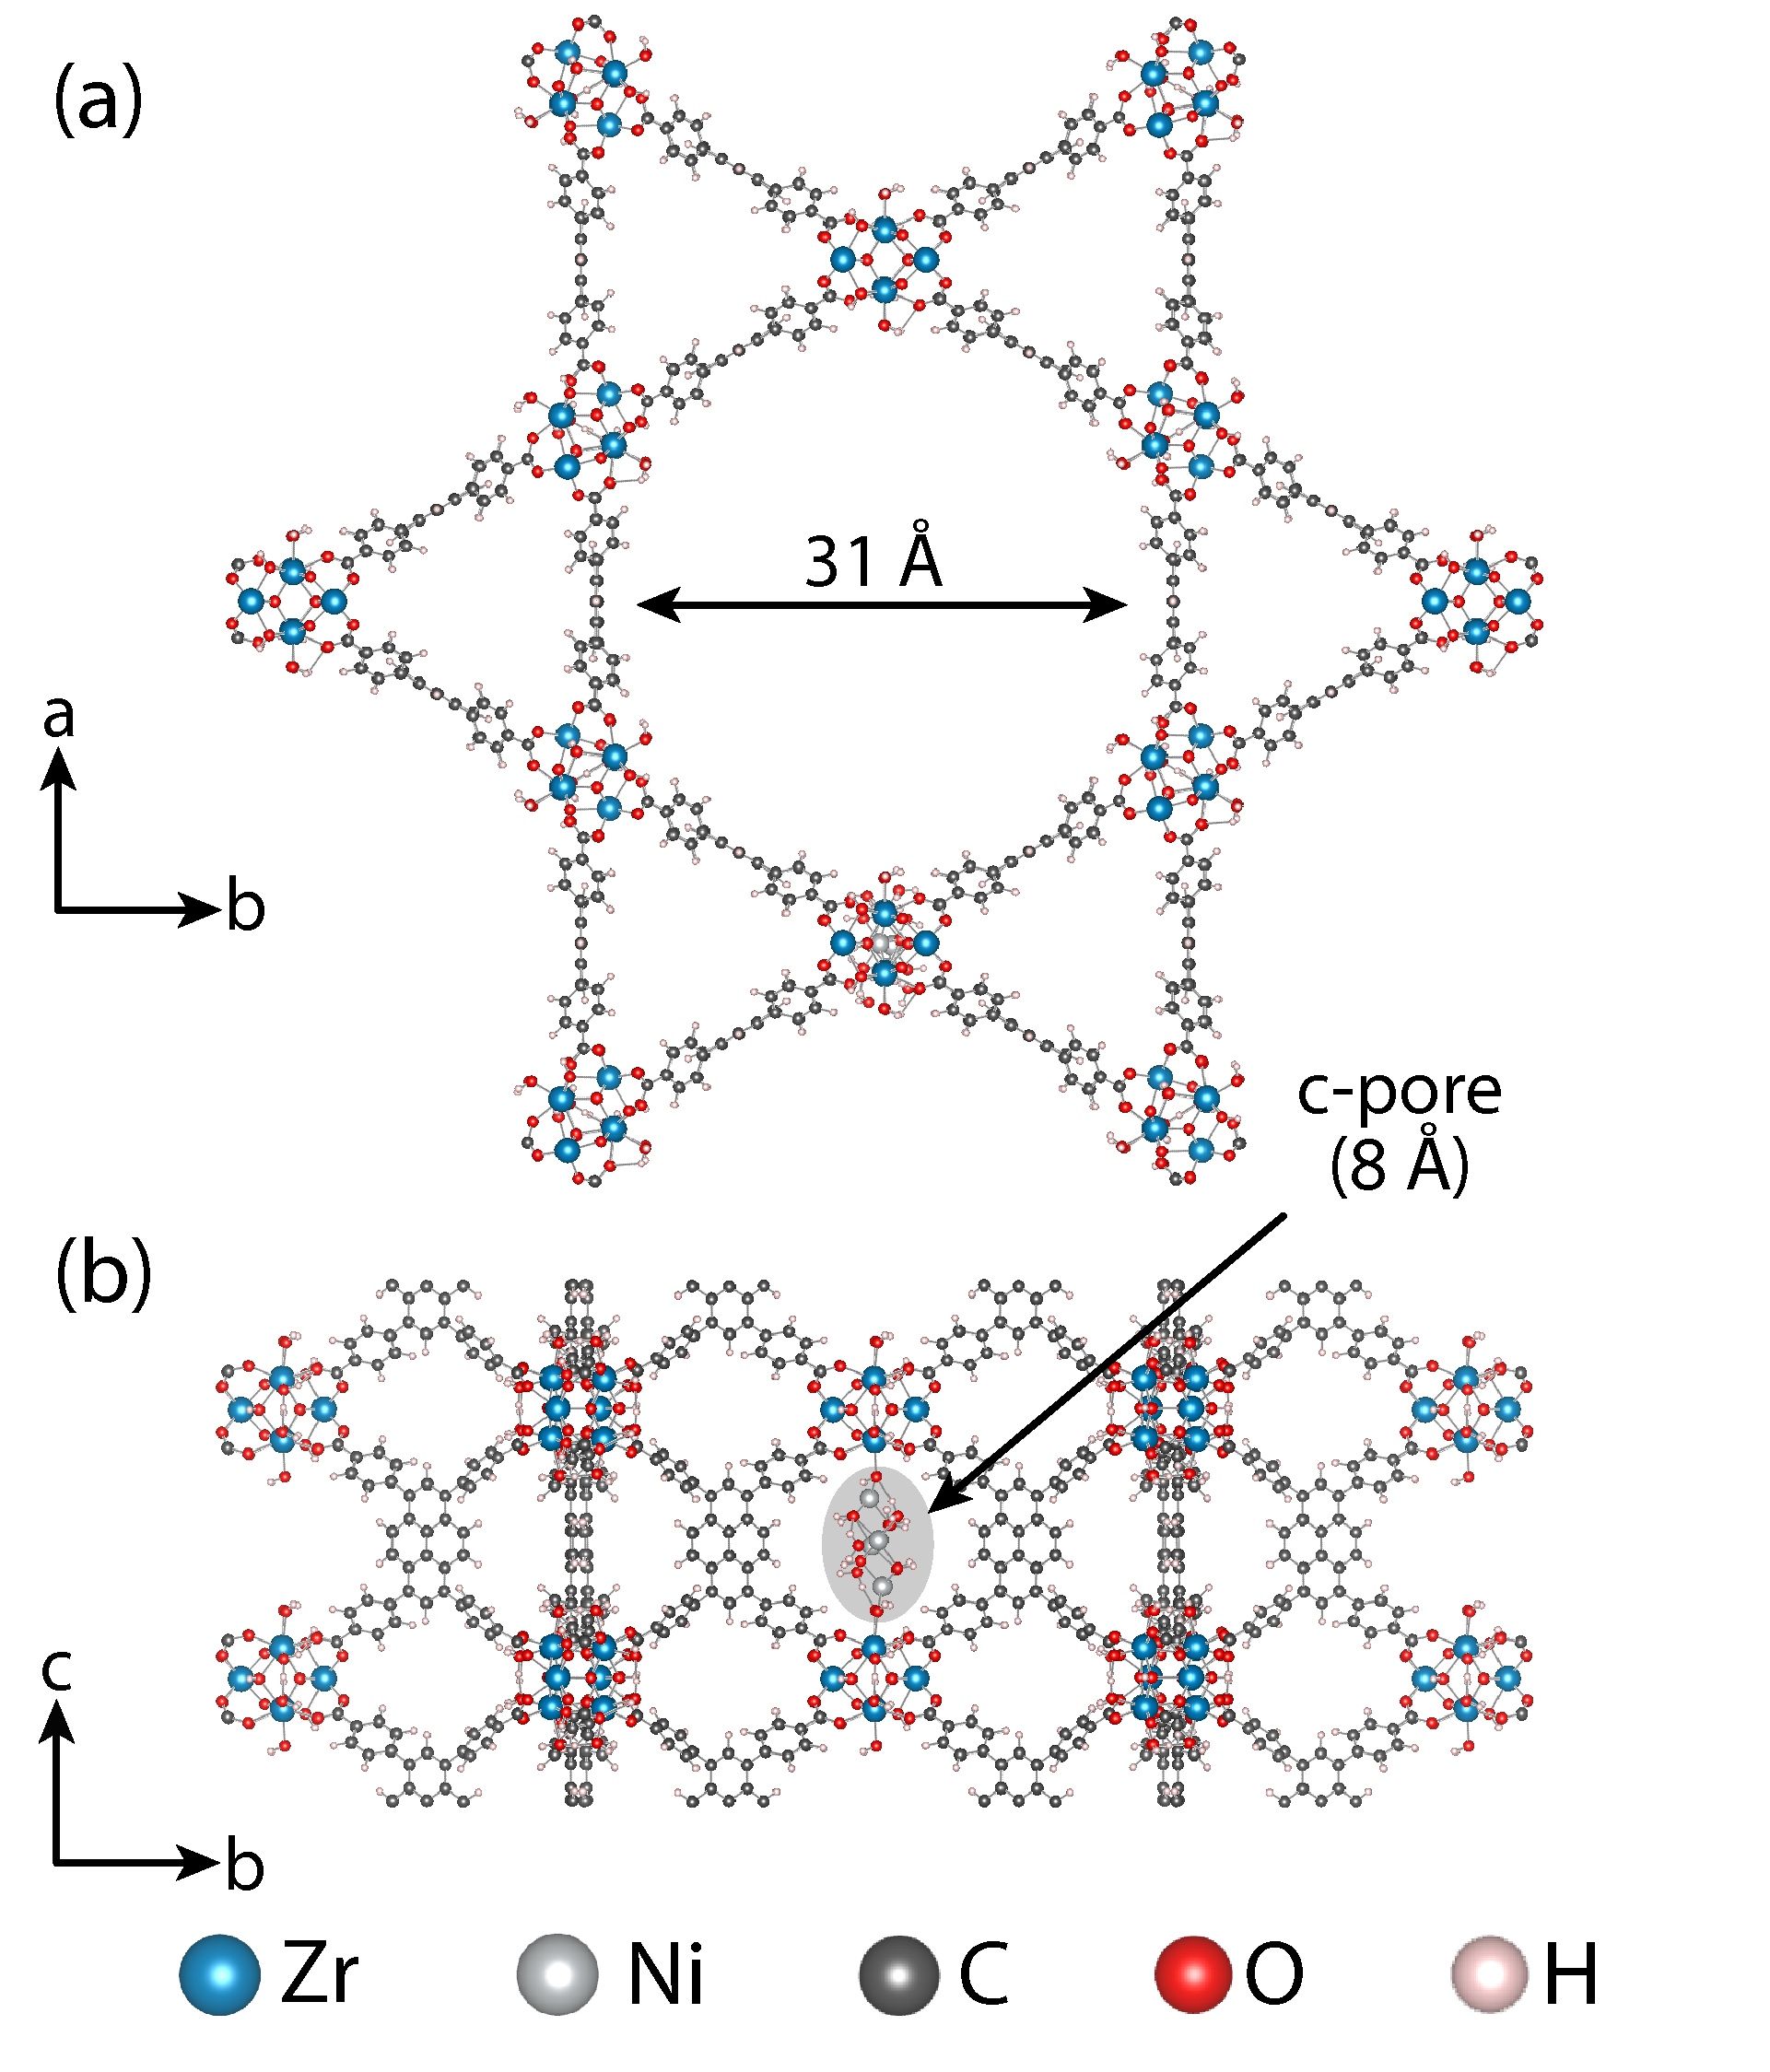
\includegraphics[width=3.0in]{zi-images/00-General-Graphics/2022-figure-MOF-schematic.png}
    \caption{
    The structure of NU-1000 shown along the (a) c-axis and the (b) a-axis with the location of the \ce{Ni} metal cluster highlighted by the gray oval. The metal cluster is located within the 8~{\AA} pore of Ni-NU-1000. The diameters of the hexagonal (31~{\AA}) and triangular (10~{\AA}) channels are also indicated.
    }
    \label{fig:Ni-MOF-model}
\end{figure}

\section{Methodology}
%%%%%%%%%%%%%%%%%%%%%%%%%%%%%%%%%%%%%%%%%%%%%%%%%%%%%%%%%%%%%%%%%%%%%
%% Methodology
%%%%%%%%%%%%%%%%%%%%%%%%%%%%%%%%%%%%%%%%%%%%%%%%%%%%%%%%%%%%%%%%%%%%%

\subsection{Differential Pair Distribution Function Analysis}

Differential pair distribution function (d-PDF) analysis is performed to reveal key interatomic distances in the Ni-NU-1000 catalysts and reveal characteristics such as coordination number and existence of ligand asymmetry. Ni-NU-1000 catalysts are synthesized using AIM as described previously.\cite{Mondloch2013, Li2016sintering} Synthesized catalysts are then exposed to \ce{H2} (3.5\% in \ce{He}) at 200 \degree C for 2 hours and then cooled to 50 \degree C in \ce{H2}.\cite{PlateroPrats2017} Powder X-ray diffraction (XRD) and total scattering data suitable for PDF analysis are then collected at 50 \degree C in \ce{H2}. PDFs are then taken using the PDFgui software;\cite{Farrow2007} details of these simulations are described in detail elsewhere.\cite{PlateroPrats2017}. PDFs represent the local structure as a histogram of atom-atom distances in the material weighted by the scattering power of the atoms involved. These are used to derive d-PDFs by subtracting the PDF measured for NU-1000 from the PDF measured for Ni-NU-1000, to isolate the atom-atom distances that define the \ce{Ni} cluster and its interaction with NU-1000 support. Of interest are the \ce{Ni{\Compactcdots}Ni} and \ce{Ni-O} distances within the cluster and the \ce{Ni{\Compactcdots}Zr} and \ce{Ni{\Compactcdots}O} distances between the cluster and NU-1000. In this notation, atom pairs not directly bonded to each other are denoted with ``${\Compactcdots}$" (given the lower scattering contribution from the \ce{O} atoms compared to \ce{Ni} atoms, \ce{O{\Compactcdots}O} pairs have very low contribution to the measured data and are not calculated.) PDFs of the computed structural models are simulated using typical values of instrument and atomic displacement parameters for such materials and then evaluated for their correspondence to the experimental data over XYZ {\AA} range.  

\subsection{Computational Details}

\subsubsection{Catalyst Structure Models}

Modeling is carried out to provide molecular level insight into the Ni-NU-1000 ligand environment. NU-1000 (P6/mmm space group) features small 8~{\AA} pores with uniform hexagonal (31~{\AA}) and triangular (10~{\AA}) channels (Figure \ref{fig:Ni-MOF-model}). DFT-optimized unit cell parameters are $a=b=40.611$ {\AA}, $c=15.990$ {\AA}, $\alpha=\beta=\ang{90}$, and $\gamma=\ang{60}$. Simulated structures contain one \ce{Ni} cluster per unit cell. Based on the current knowledge about Ni-NU-1000 catalysts,\cite{PlateroPrats2017} these clusters comprise four \ce{Ni} ions and span the small pores of NU-1000, connecting two adjacent nodes (Figure~\ref{fig:Ni-MOF-model}b). (Structures comprising fewer than four \ce{Ni} ions were also evaluated, but gave poor agreement with the experimental d-PDF; see \hl{Supporting Information Section XXX}.) Clusters bind to the nodes by replacing two protons (one on each node).\cite{Ye2017} To provide molecular-level insight into the types of ligand environments that could lead to the experimentally observed d-PDFs, we consider \hl{854} different structures comprising a variety of ligand environments, including hydroxyl (\ce{OH}), water (\ce{H2O}), hydride (\ce{H}), and oxygen (\ce{O}), giving stoichiometries of \ce{Ni_4O_xH_y} for all clusters considered. Four example structures are shown in Figure~\ref{fig:Ni-MOF-structures}. The full library of structures considered in this work can be accessed on our GitHub page.\cite{GitHub-Ni4Project}

\begin{figure}
    \centering
    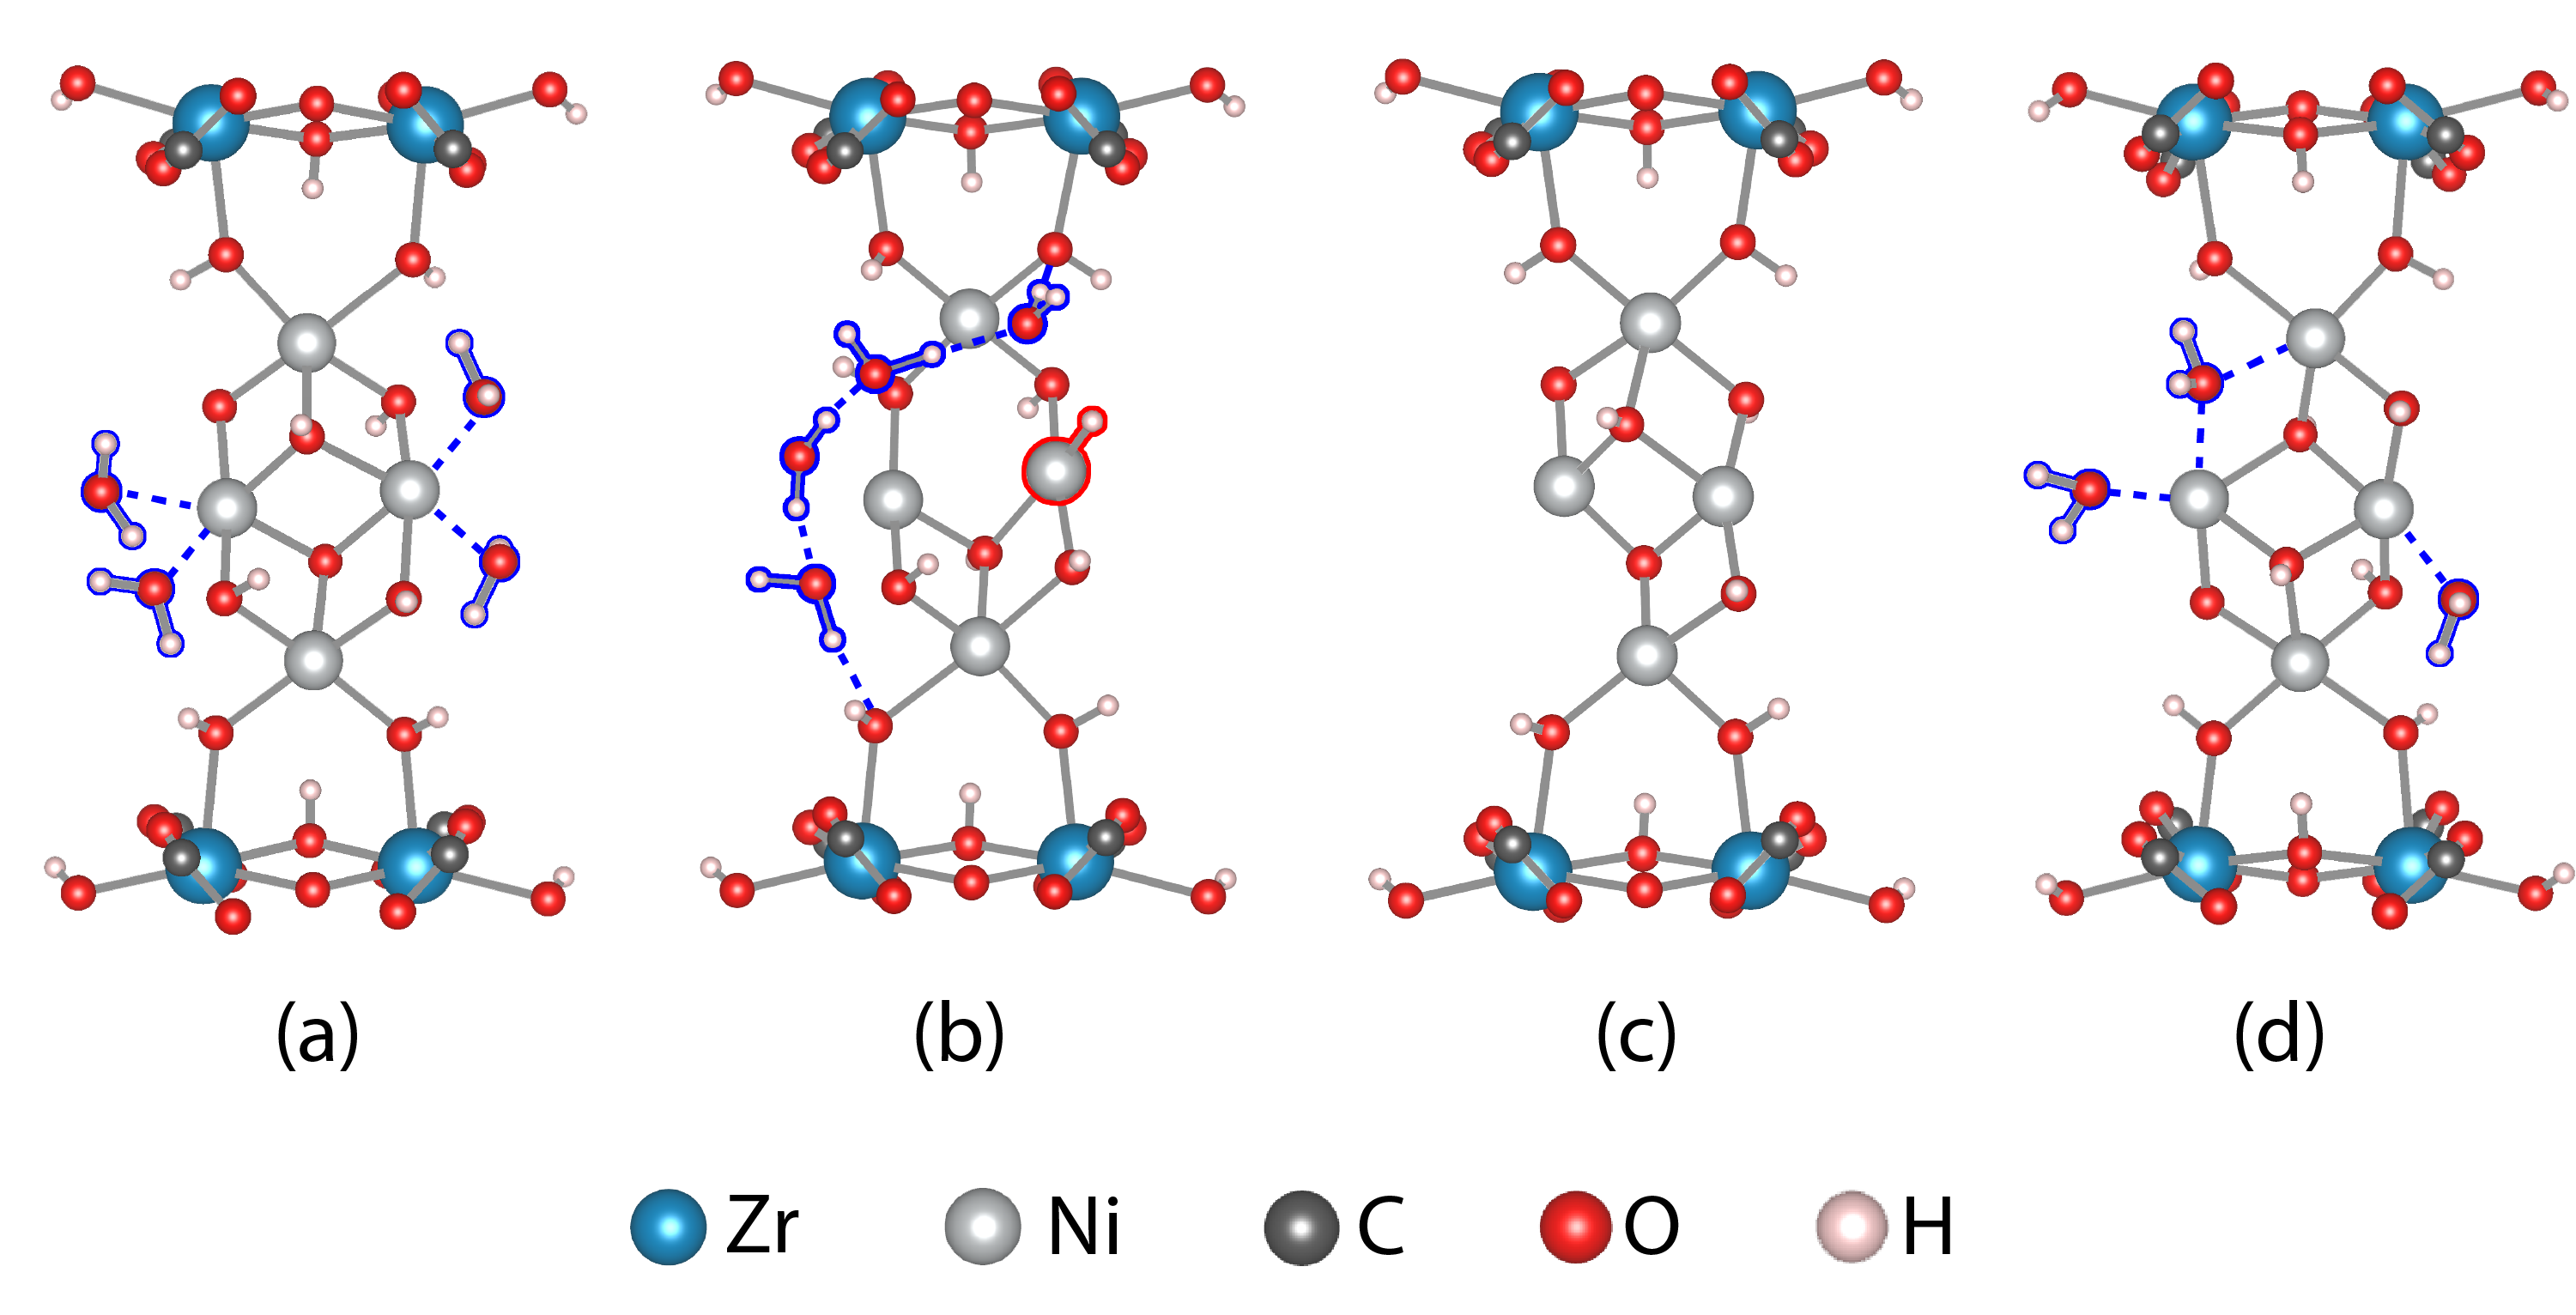
\includegraphics[width=5.0in]{zi-images/00-General-Graphics/2022-figure-clusters-3xstructures.png}
    \caption{
    Some of the \ce{Ni_4O_xH_y} clusters evaluated in this work. (a) \ce{Ni4(OH)6.4H2O} (green), (b) \ce{Ni4(OH)5(H).4H2O} (blue), (c) \ce{Ni4(OH)4(O)} (yellow), and (d) \ce{Ni4(OH)4(O).3H2O} (maroon). Colors in parentheses are the same as for Figures~\ref{fig:phase_diagram_Ni} and \ref{fig:Ni-structure-diagram}. The NU-1000 structure is excluded from the pictures for clarity, except for the \ce{Zr} ions where the clusters are attached. The atom color key is indicated in the figure. \ce{H2O} molecules and ligands are outlined in blue, and \ce{Ni-H} ligands are outlined in red.
    }
    \label{fig:Ni-MOF-structures}
\end{figure}

\subsubsection{\textit{ab initio} Thermodynamics Modeling}

\textit{ab initio} thermodynamic analysis\cite{Reuter2003, Reuter2004, Grundner2015, Paolucci2016, Li2016, Getman2008, Mandal2020, Zuo2016, Tang2019} is used to determine the thermodynamically stable structures as functions of chemical potential (which can be related to gas phase temperature and partial pressure using an equation of state; \hl{see Supporting Information} Section \hl{XXX}). We specifically consider chemical potentials of \ce{H2} (g) ($\mu_{\ce{H2}}$) and \ce{H2O} (g) ($\mu_{\ce{H2O}}$). \ce{H2} (g) is chosen since experimental d-PDFs were collected under hydrogenation conditions. \ce{H2O} (g) is chosen since we find hydrogen atom binding on the cluster often occurs on hydroxyl ligands, forming \ce{H2O} ligands, which can then desorb. \ce{H2O} (g) is hence a convenient oxygen reference.  Cluster free energies are then calculated as:
\begin{equation}
    \begin{split}
        \Delta F^{(2)}(V,T,\mu_{\text{H}},\mu_{\text{O}},N_{\text{Ni}})  
        & = \Delta F(V,T,N_{\text{H}},N_{\text{O}},N_{\text{Ni}}) - (\mu_{\text{H}})(\Delta N_{\text{H}}) \\
        & - (\mu_{\text{O}})(\Delta N_{\text{O}})  \\ 
    \end{split}
    \label{eq:free-energy-trans}
\end{equation}
where $F^{(2)}$ is the the second Legendre transform of the Helmholtz free energy (i.e., of $N_{\ce{H}}$ and $N_{\ce{O}}$ to $\mu_{\ce{H}}$ and $\mu_{\ce{O}}$),\cite{Alberty1997} $V$ is volume, $T$ is temperature, $\mu$ is chemical potential, and $N$ is number, i.e., of \ce{O} and \ce{H} atoms within the cluster. $\mu_{\ce{H}} = \frac{1}{2} \mu_{\ce{H}_2}$, and $\mu_{\text{O}} = \mu_{\ce{H2O}} - 2\mu_{\ce{H}}$. $F = E^\text{elec} + E^\text{ZP} + F^\text{vib}$, where $E^\text{elec}$ is the electronic energy calculated with DFT, $E^\text{ZP}$ is the zero point vibrational energy, and $F^\text{vib}$ is the temperature dependent vibrational free energy. The $\Delta$'s in Eq.~\ref{eq:free-energy-trans} indicate quantities taken relative to a reference structure; the reference structure used in this work is the \ce{Ni4(OH)6.4H2O} structure shown in Figure~\ref{fig:Ni-MOF-structures}a. This structure comprises \ce{OH} and \ce{H2O} ligands (outlined in blue in Figure~\ref{fig:Ni-MOF-structures}) and is highly symmetric.

\subsubsection{Density Functional Theory Calculations}
Electronic energies are calculated using the CP2K software package\cite{Hutter2014} using the PBE exchange and correlation functional\cite{Perdew1996}, damped D3 dispersion corrections,\cite{Grimme2010} the DZVP-MOLOPT basis set,\cite{VandeVondele2007} and Goedecker pseudopotentials.\cite{Goedecker1996} Plane waves are simulated up to 360 Ry. As a single divalent \ce{Ni} ion can adopt singlet or triplet spin states, we evaluate singlet, triplet, quintet, septet, and nonet states for the \ce{Ni4} clusters, following prior work.\cite{Shabbir2020, Ye2017, Bernales2016} The Unrestricted Kohn-Sham (UKS) method is employed given the open shell nature of the system. Spin states exhibiting spin contamination are not considered in \textit{ab initio} thermodynamic analysis. Details about how spin contamination is determined and the criteria used to keep or discard structures is provided in Supporting Information Section \hl{XXX}. Electronic energies are obtained from geometry relaxations where all atoms in the periodic unit cell are allowed to relax. $E^\text{ZP}$ and $F^\text{vib}$ are calculated from the calculated vibrational modes. Details about how the vibrational modes, $E^\text{ZP}$, and $F^\text{vib}$ are calculated are provided in \hl{Supporting Information}. Vibrational modes are only calculated for structures within 100 kJ/mol of the lowest electronic-energy cluster at each unique composition to decrease computational expense, with a few exceptions discussed below. Details about how $E_{\text{H}_2}$ and $E_{\text{H}_2\text{O}}$ are calculated and sample CP2K input files for all types of DFT calculations carried out in this work are provided in Supporting Information. 

\section{Results and Discussion}
%%%%%%%%%%%%%%%%%%%%%%%%%%%%%%%%%%%%%%%%%%%%%%%%%%%%%%%%%%%%%%%%%%%%%
%% Results 
%%%%%%%%%%%%%%%%%%%%%%%%%%%%%%%%%%%%%%%%%%%%%%%%%%%%%%%%%%%%%%%%%%%%%

% d-PDF Diagram
\begin{figure}
    \centering
    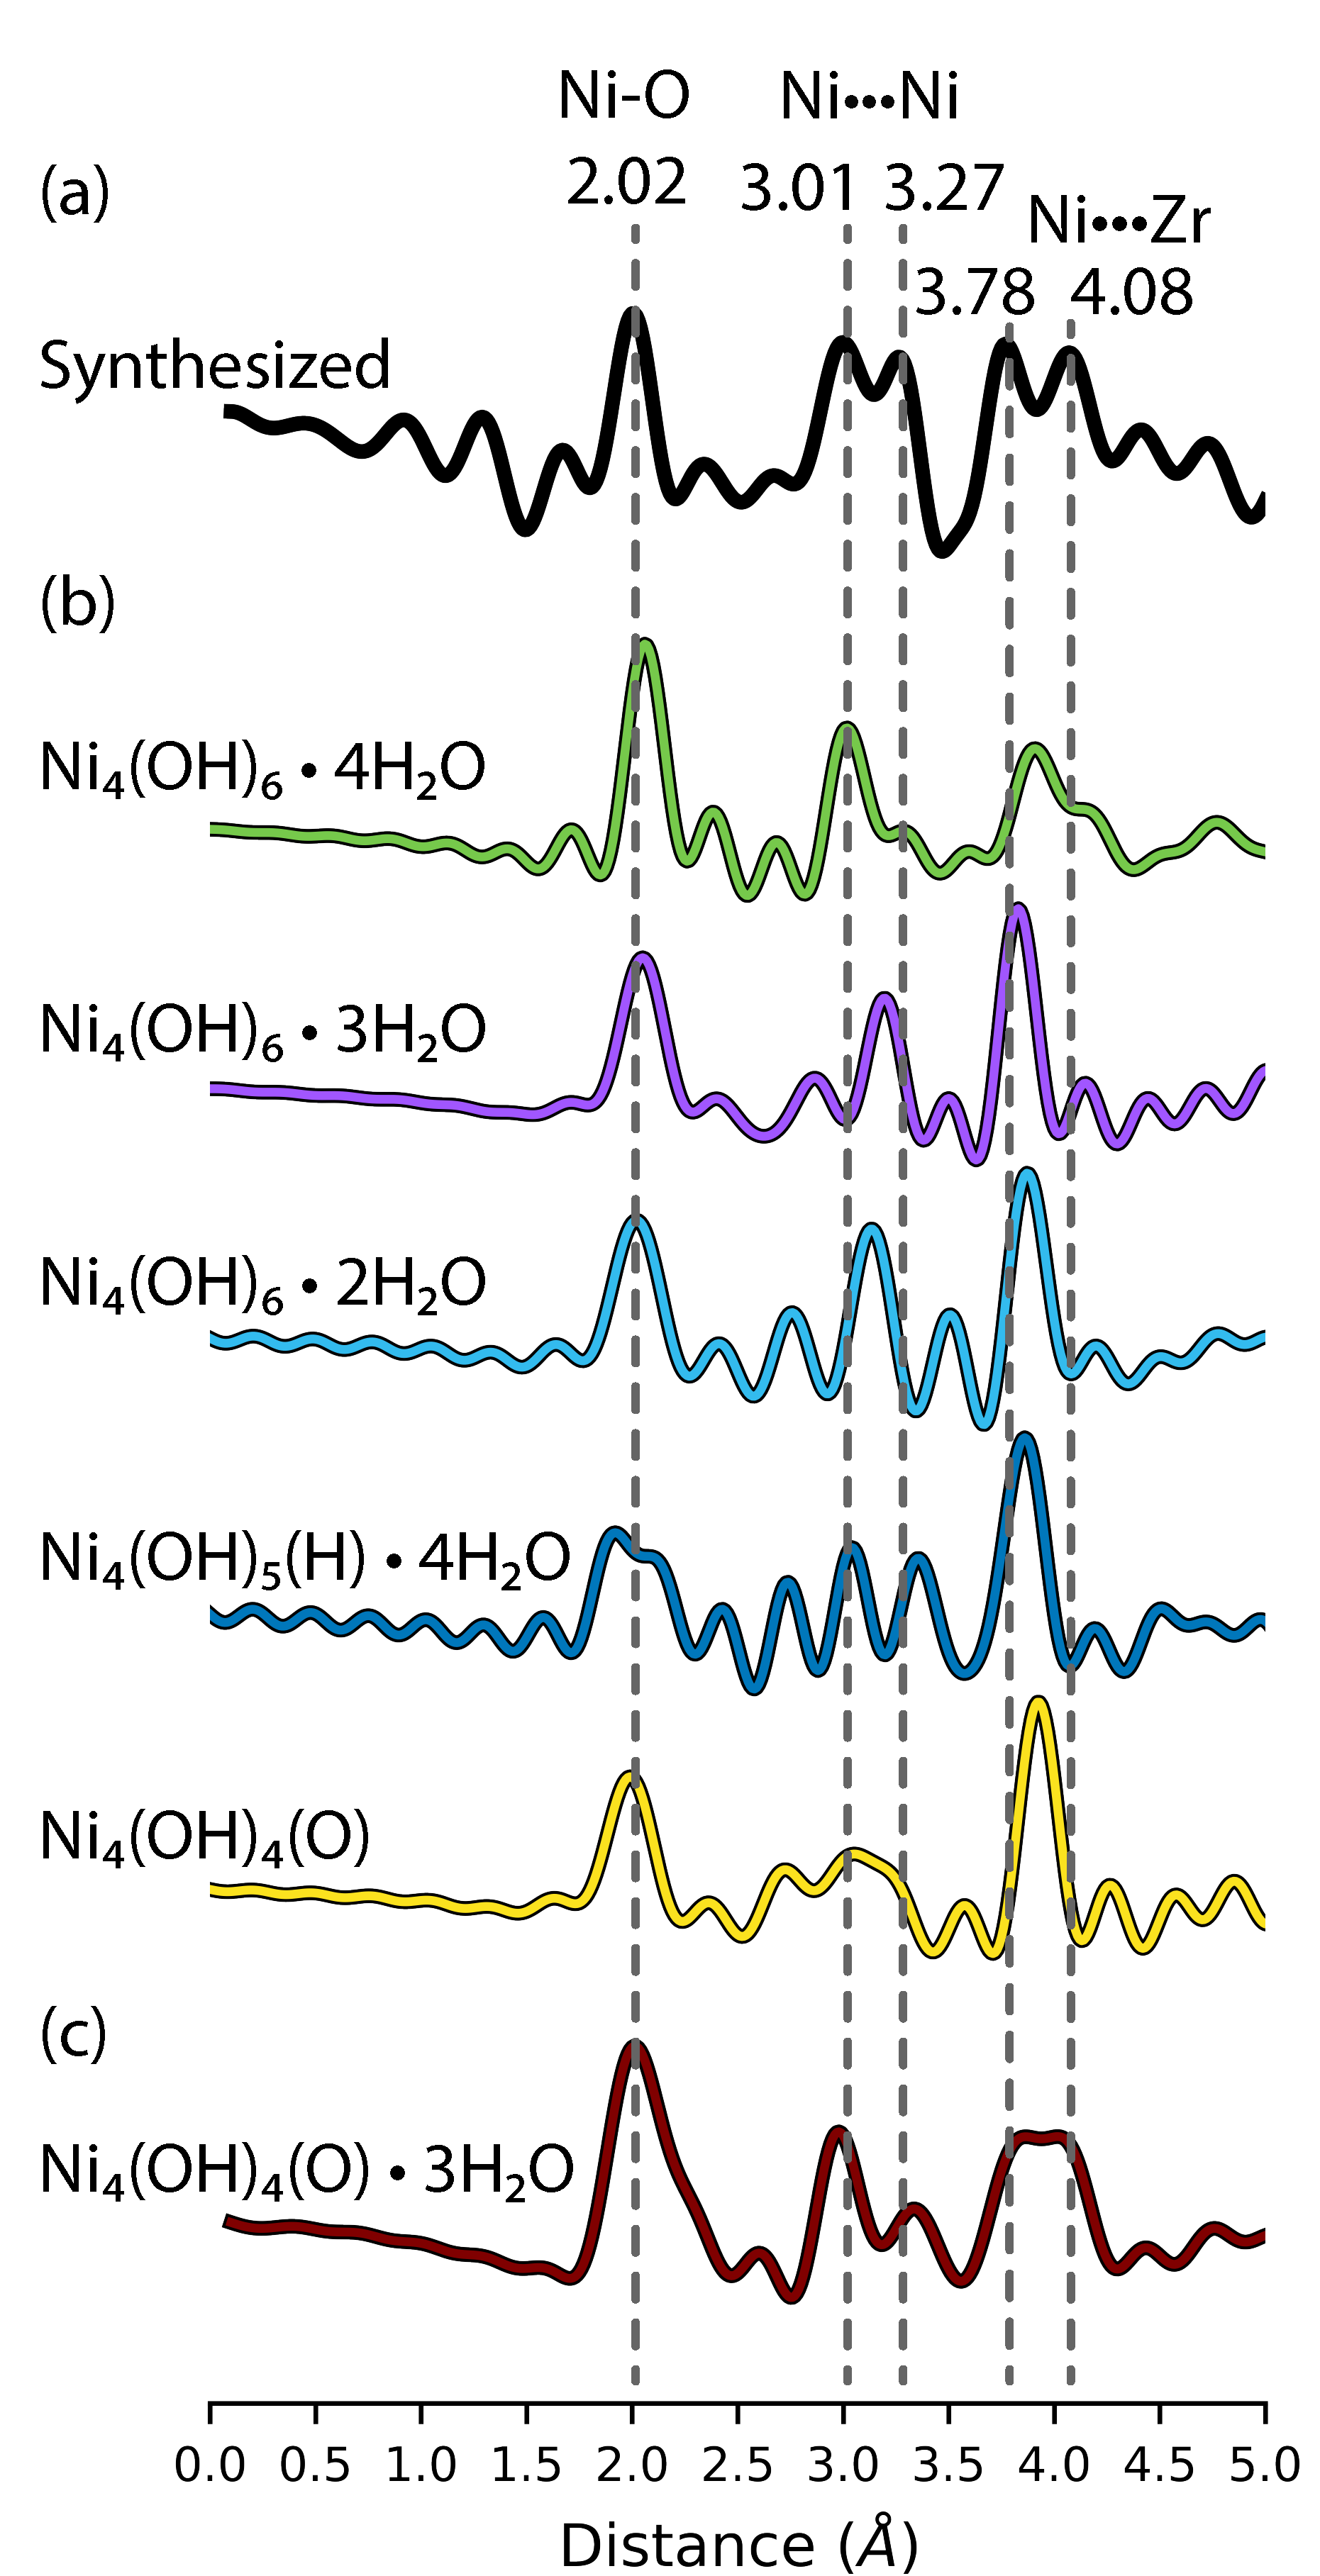
\includegraphics{zi-images/01-Ni-Graphics/2021-MAIN-single-dPDF.png}
    \caption{
    d-PDFs for (a) the synthesized structure, (b) simulated structures representing thermodynamic minima with \ce{Ni-O} coordination numbers $\ge$ 4, and (c) the simulated structures that give the best agreement with the synthesized structure. Structure labels and colors for the simulated structures are the same as in the text and in Figures~\ref{fig:phase_diagram_Ni} and \ref{fig:Ni-structure-diagram}. Gray dotted lines indicate key distances observed for the synthesized structure, which are also annotated on the figure.
    }
    \label{fig:dPDFs-graphic}
\end{figure}

The d-PDF for the synthesized Ni-NU-1000 catalyst is shown in Figure~\ref{fig:dPDFs-graphic}a.\cite{PlateroPrats2017} Key peaks are the single peak at 2.02 {\AA}, split peaks at 3.01 {\AA} and 3.27 {\AA}, and split peaks at 3.78 {\AA} and 4.08 {\AA}, which correspond to \ce{Ni-O}, \ce{Ni{\Compactcdots}Ni}, and \ce{Ni{\Compactcdots}Zr} distances, respectively. Prior work indicates that the \ce{Ni-O} coordination number is $\sim$5.\cite{PlateroPrats2017} 

Figure~\ref{fig:phase_diagram_Ni} plots a phase diagram constructed using \textit{ab initio} thermodynamic analysis that indicates the thermodynamically most stable structures within the simulated database. In this phase diagram, the different colored regions correspond to different structures, which are depicted in Figure~\ref{fig:Ni-structure-diagram}. Each structure is annotated with its \ce{Ni-O} coordination number; ranges of $\mu_{\ce{H2}}$ and $\mu_{\ce{H2O}}$ are selected such that coordination numbers $\sim$5 are centered in order to match experimental findings. (Expansion of the phase diagram to higher and lower values of $\mu_{\text{H}_2\text{O}}$ and $\mu_{\text{H}_2}$ does not reveal any additional structures or higher coordination numbers; See \hl{Supporting Information Section XX} for further details.) The structures \ce{Ni4(OH)6.2H2O} (cyan), \ce{Ni4(OH)6.3H2O} (purple), and \ce{Ni4(OH)6.4H2O} (green) give \ce{Ni-O} coordination numbers of 4.5, 5.0, and 5.5, which are in line with the experimentally observed value of $\sim$5. These structures comprise significant \ce{OH} and \ce{H2O} ligands and no \ce{O} or \ce{H} ligands and have stoichiometries of \ce{Ni4O8H10}, \ce{Ni4O9H12}, and \ce{Ni4O10H14}, respectively. They reside on the phase diagram at higher (more positive) values of $\mu_{\text{H}_2\text{O}}$ and lower (more negative) values of $\mu_{\text{H}_2}$. As these structures in agreement with the experimentally observed \ce{Ni-O} coordination number are stable at higher values of $\mu_{\text{H}_2\text{O}}$, which correspond to larger \ce{H2O} concentrations (and lower temperatures), this finding suggests that NU-1000 comprises significant \ce{H2O} concentration, even after exposure to \ce{H2}/\ce{He} at 200 \degree C for 2 hours and measurement in \ce{H2}/\ce{He} at 50 \degree C. Similar \ce{H2O} storage properties have been observed in MOF-303\cite{Hanikel2021} and MOF-801\cite{Kim2017} under ambient conditions. The vertical dotted line in Figure~\ref{fig:Ni-structure-diagram} indicates values of $\mu_{\ce{H2}}$ used during collection of the experimental d-PDF. The structures \ce{Ni4(OH)6.3H2O} (purple) and \ce{Ni4(OH)6.4H2O} (green) fall along this line and have significant \ce{OH} and \ce{H2O} content. 

% Phase Diagram
\begin{figure}[H]
    \centering
    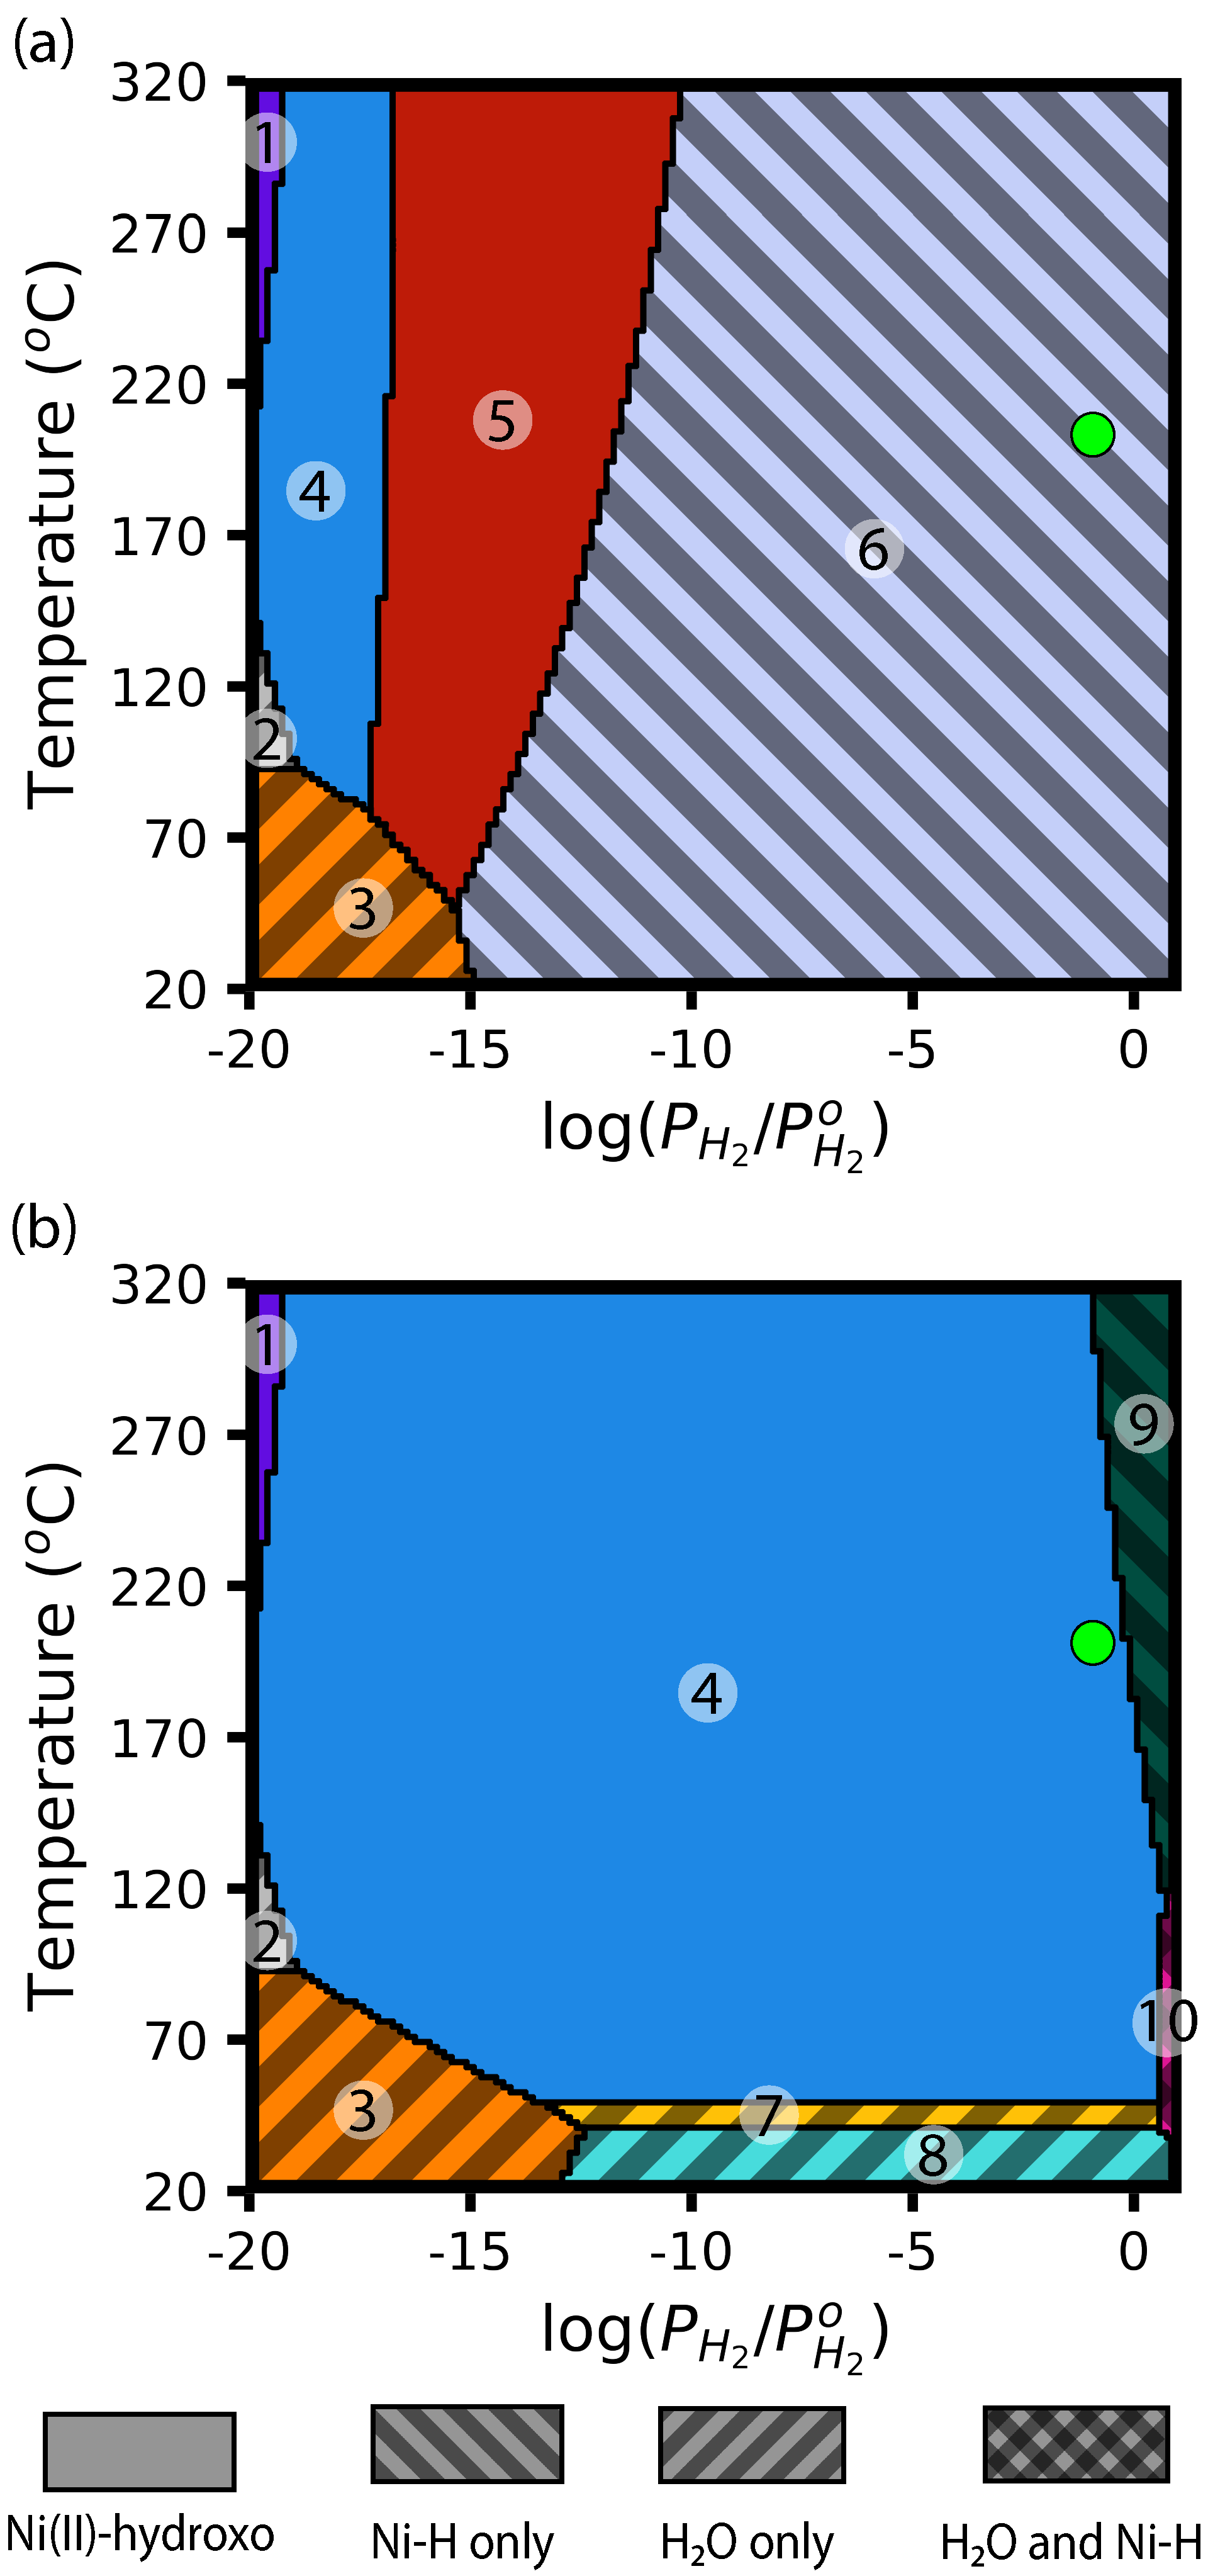
\includegraphics{zi-images/01-Ni-Graphics/2021-MAIN-phase-diagram-combined.png}
    \caption{
    Calculated phase diagram for the \ce{Ni4} cluster presented as a function of $\Delta \mu_{\ce{H2}}$ and $\Delta \mu_{\ce{H2O}}$, where the $\Delta$'s indicate the values are referenced to the 0~K values (derivation provided in Supporting Information). The different colored regions indicate different structures and follow the same key as in Figures~\ref{fig:dPDFs-graphic} and \ref{fig:Ni-structure-diagram}. The numbers indicate the \ce{Ni-O} coordination number. The hash patterns indicate the types of ligand environments and follow the key in the figure. The vertical dashed line indicates the value of $\Delta \mu_{\text{H}_2}$ corresponding to the conditions where the experimental d-PDF was collected (\ce{H2} in 3.5\% in \ce{He} at 50 \degree C and ambient pressure). As \ce{H2O} was not added in experiments, values of $\Delta \mu_{\ce{H2O}}$ are chosen such that the \ce{Ni-O} coordination number matches the experimentally observed value of $\sim$5 (e.g., $\Delta \mu_{\ce{H2O}} > \sim -40$ along the vertical dashed line). Structures with \ce{Ni-O} coordination numbers $\ge$ 4.0 are \ce{Ni4(OH)4(O)} (yellow; 4.0), \ce{Ni4(OH)5(H).4H2O} (blue; 4.3), \ce{Ni4(OH)6.2H2O} (cyan; 4.5), \ce{Ni4(OH)6.3H2O} (purple; 5.0), and \ce{Ni4(OH)6.4H2O} (green; 5.5).
    }
    \label{fig:phase_diagram_Ni}
\end{figure}  

% Structure Diagram
\begin{figure}
    \centering
    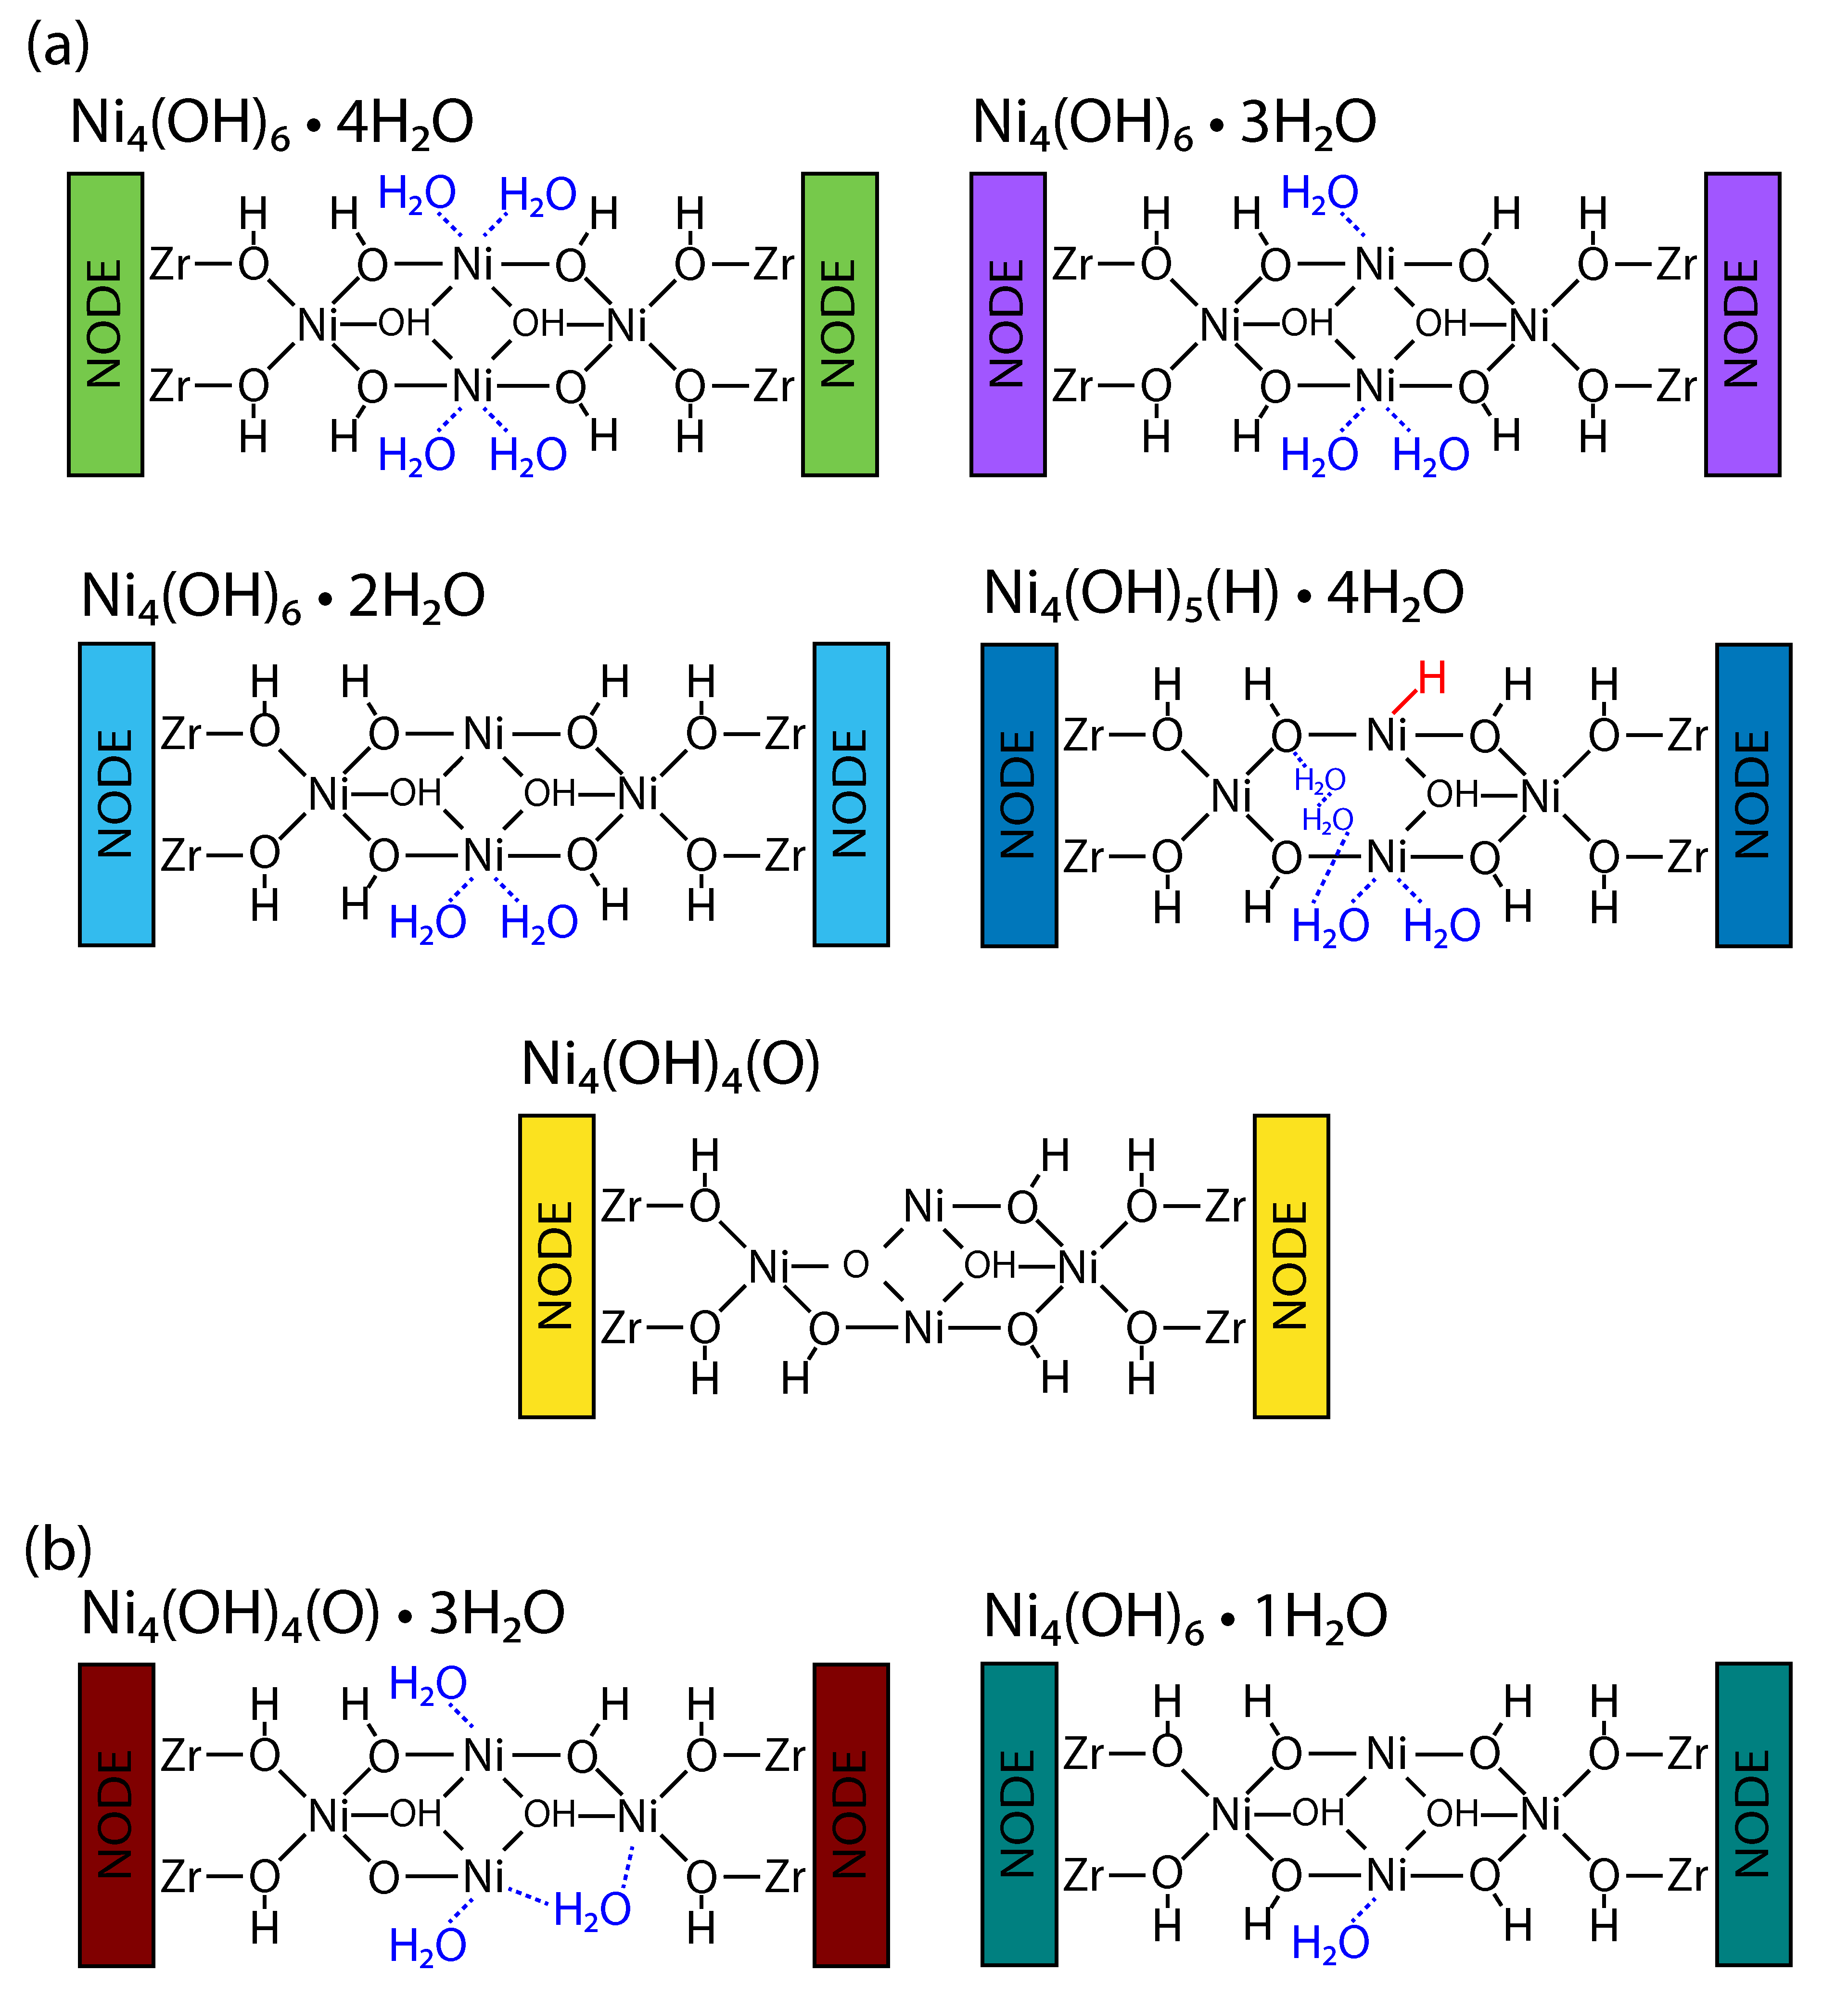
\includegraphics[width=0.75\textwidth]{zi-images/01-Ni-Graphics/2021-MAIN-structure-diagram.png}
    \caption{
    Depictions of (a) structures from Figure~\ref{fig:phase_diagram_Ni} with \ce{Ni-O} coordination numbers $\ge$ 4 and (b) the structures that exhibit d-PDFs that give the best agreement with that of the synthesized structure. The color scheme is the same as in Figures~\ref{fig:dPDFs-graphic} and \ref{fig:phase_diagram_Ni}. \ce{H2O} molecules and ligands are indicated with blue text, and \ce{Ni} hydrides are indicated with red text for emphasis. Color code: Part a: Top row: green (left), purple (right). Second row: cyan (left), blue (right). Third row: yellow. Part b: teal (left), maroon (right).  
    }
    \label{fig:Ni-structure-diagram}
\end{figure}

To compare with experiment, d-PDFs for all structures on the phase diagram with \ce{Ni-O} coordination numbers $\ge$ 4 are shown in Figure~\ref{fig:dPDFs-graphic}b. We seek structures that give good agreement with the \ce{Ni-O} and \ce{Ni{\Compactcdots}Ni} peaks seen in the experimental d-PDF, as matching these peak positions provides insights into the ligand environments of the \ce{Ni} ions. \ce{Ni-O} peaks in general agree well with experiment, except for \ce{Ni4(OH)5(H).4H2O} (blue), which exhibits asymmetric split peaks instead of a single peak. From Figure~\ref{fig:Ni-structure-diagram}, this asymmetry is likely caused by an asymmetric ligand environment (Figure~\ref{fig:Ni-MOF-structures}b). Specifically, in addition to \ce{OH} and \ce{H2O} ligands, the \ce{Ni4(OH)5(H).4H2O} (blue) structure comprises a Ni hydride (\ce{H} ligand) as well as a bridge of \ce{H2O} molecules that connect one \ce{Ni} ion with a \ce{OH} ligand on the opposite side of the cluster. That asymmetry in the \ce{Ni-O} peak is not observed experimentally indicates that the ligand environments on the different \ce{Ni} ions in the synthesized structure are more symmetric than those in structure \ce{Ni4(OH)5(H).4H2O} (blue).  

There is less agreement between simulations and experiments for the \ce{Ni{\Compactcdots}Ni} peaks in the d-PDFs in Figure~\ref{fig:dPDFs-graphic}. In the experimental d-PDF, these peaks are split, suggesting that there is at least some asymmetry and/or disorder in the cluster; however, most of the simulated structures exhibit a single \ce{Ni{\Compactcdots}Ni} peak. The exceptions are \ce{Ni4(OH)5(H).4H2O} (blue) and \ce{Ni4(OH)4(O)} (yellow), which are shown in Figures~\ref{fig:Ni-MOF-structures}b and c respectively. While \ce{Ni4(OH)5(H).4H2O} (blue) exhibits a highly asymmetric ligand environment including a \ce{H2O} molecule chain and a \ce{Ni} hydride, \ce{Ni4(OH)4(O)} (yellow) comprises mainly \ce{OH} ligands and one \ce{O} ligand (but no \ce{H2O} or \ce{H} ligands). Taken together, these comparisons suggest that the synthesized catalyst could exhibit a mix of \ce{OH}, \ce{H2O}, and \ce{O} ligands.

Alternatively, the observed d-PDF could be due to a distribution of multiple structures present under collection conditions. Whereas the phase diagram only presents the simulated structure with the lowest free energy, other structures that are similar in energy could be present experimentally and hence contribute to the observed d-PDFs. To test this hypothesis, we created a d-PDF based off multiple simulated structures, with the different contributions dictated by their relative Boltzmann weights (details provided in \hl{Supporting Information Section XXX}). These d-PDFs are calculated at various chemical potentials and are presented in Figure S\hl{XXX}. We find that weighting has a large contribution to the simulated d-PDF at $\mu_{\text{H}_2\text{O}}$ and $\mu_{\text{H}_2}$ near the boundaries between structures on the computed phase diagram. For example, the weighted d-PDF near the boundary between the \ce{Ni4(OH)6.4H2O} (green) and \ce{Ni4(OH)6.3H2O} (purple) structures exhibits a significantly broadened \ce{Ni{\Compactcdots}Ni} peak (Figure~S\hl{XXX}c). The \ce{Ni4(OH)6.4H2O} (green) and \ce{Ni4(OH)6.3H2O} (purple) structures differ by a single \ce{H2O} ligand and exhibit different \ce{Ni{\Compactcdots}Ni} peak positions as shown in Figure~\ref{fig:dPDFs-graphic}b, suggesting that the split \ce{Ni{\Compactcdots}Ni} peaks observed experimentally could be due to a slight difference in \ce{H2O} content amongst clusters in the experimental structure. 

Another possible explanation is that errors in the computational methods prevent structural matching between experiments and theory, i.e., by predicting one structure to have the lowest free energy whereas a different structure is observed experimentally. To investigate this, we generated d-PDFs for the remaining structures in the simulated database (i.e., for the remaining structures not included in Figure~\ref{fig:phase_diagram_Ni}). For example, the \ce{Ni4(OH)6.1H2O} (teal) structure, depicted in Figure~\ref{fig:Ni-structure-diagram}b, exhibits split \ce{Ni{\Compactcdots}Ni} peaks (see Figure~\ref{fig:dPDFs-graphic}c). This structure features a single \ce{H2O} ligand coordinated to one of the \ce{Ni} ions, suggesting that even slight asymmetries in the coordination environment can lead to split \ce{Ni{\Compactcdots}Ni} peaks. The \ce{Ni4(OH)6.1H2O} (teal) structure is at least $\sim$170~kJ/mol higher in free energy than any structure on the phase diagram, depending on $\mu_{\ce{H2O}}$ and $\mu_{\ce{H2}}$, which is much greater than the typical error associated with DFT-based methods (of $\sim$30~kJ/mol), so it is unlikely that it is contributing to the observed d-PDF; however, the fact that one \ce{H2O} ligand leads to split \ce{Ni{\Compactcdots}Ni} peaks in the d-PDF is in agreement with the analysis on Boltzmann weighting described above. Taken together, these results suggest that the split \ce{Ni{\Compactcdots}Ni} peaks could be caused by different numbers of \ce{H2O} ligands on the different \ce{Ni} ions in the experimental catalyst.  

The last remaining feature of the d-PDFs is the \ce{Ni{\Compactcdots}Zr} peak. As for the \ce{Ni{\Compactcdots}Ni} peak, the experimental structure exhibits split peaks whereas the structures on the phase diagram exhibit a single peak. Searching back through the simulated database, we find that the \ce{Ni4(OH)4(O).3H2O} (maroon) structure, which is depicted in Figures~\ref{fig:Ni-MOF-structures}d and \ref{fig:Ni-structure-diagram}b, exhibits broad \ce{Ni{\Compactcdots}Zr} peaks. This structure comprises an asymmetric mixture of \ce{OH}, \ce{H2O}, and \ce{O} ligands, including one \ce{H2O} molecule that bridges two Ni ions, one of which also binds to an \ce{OH} ligand that is also connected to \ce{Zr} (Figure~\ref{fig:Ni-MOF-structures}d), analogous to the \ce{\mu_{2}OH} ligands seen in the other structures (Figure~\ref{fig:Ni-structure-diagram}). The \ce{Ni4(OH)4(O).3H2O} (maroon) structure is at least $\sim$350~kJ/mol higher in free energy than any structure on the phase diagram, so it unlikely contributes to the observed d-PDF; however, it again suggests \ce{H2O} ligands as a possible reason for the observed peak splitting. Alternatively, the split peaks could be caused by unit cell asymmetry caused by node distortions, which has been previously observed for NU-1000 during \ce{Ni} deposition and under conditions relevant for catalytic hydrogenation.\cite{PlateroPrats2016} 

Taken together, all of these results suggest significant \ce{H2O} content in Ni-NU-1000 as well as significant \ce{H2O} ligands on the Ni cluster. Further, asymmetric arrangements of \ce{H2O} ligands and/or distributions of clusters with slightly different \ce{H2O} contents could lead to the d-PDFs observed experimentally. Interestingly, only one structure comprising a \ce{Ni} hydride, i.e., structure \ce{Ni4(OH)5(H).4H2O} (blue), appears on the phase diagram. While this structure exhibits some characteristics in agreement with the synthesized structure, including split \ce{Ni{\Compactcdots}Ni} and \ce{Ni{\Compactcdots}Zr} peaks, it also exhibits split \ce{Ni-O} peaks, which is not observed experimentally, likely due to the significantly different ligand environment created by the hydride itself. These results suggest that if structures with hydride ligands exist in the experimental structure, they are present in relatively low amounts (compared to structures with \ce{OH}, \ce{O}, and especially \ce{H2O} ligands). Alternatively, hydrides may be transient, as hypothesized by \citeauthor{Li2016sintering} Alternatively, the active site could be a Ni coupled with \ce{O}/\ce{OH} or \ce{OH}/\ce{H2O} ligands, as proposed by \citeauthor{Shabbir2020} Further simulations are needed to clarify these details. Such simulations are a focus of our ongoing work.    

\section{Conclusions}
%%%%%%%%%%%%%%%%%%%%%%%%%%%%%%%%%%%%%%%%%%%%%%%%%%%%%%%%%%%%%%%%%%%%%
%% Conclusions  
%%%%%%%%%%%%%%%%%%%%%%%%%%%%%%%%%%%%%%%%%%%%%%%%%%%%%%%%%%%%%%%%%%%%%

The ligand environment of a \ce{Ni} cluster supported in the MOF NU-1000 is explored using a combination of experiments and simulations. Prior results indicate that the \ce{Ni-O} coordination number is $\sim$5. We find that clusters that exhibit such high coordination comprise a significant number of \ce{OH} and \ce{H2O} ligands and are only achievable under appreciable \ce{H2O} chemical potential. Given that experiments were performed under reducing conditions, this suggests that NU-1000 has significant \ce{H2O} storage capacity. Comparisons of experimental and simulated d-PDFs indicate that either \ce{Ni} ions within the clusters exhibit different numbers of \ce{H2O} ligands or that there is a distribution of \ce{Ni} clusters within Ni-NU-1000 that exhibit different \ce{H2O} contents. Our results also suggest that clusters comprising hydride ligands do not contribute to the observed d-PDF, meaning that if \ce{Ni-H} participate in the hydrogenation mechanism on Ni-NU-1000 catalysts, they exist in a relatively low amount that is not easily detectable in the d-PDF analysis. Further simulations are needed to clarify the active site on Ni-NU-1000 catalysts, which is a topic of our ongoing work.  

\section{References}

%The class makes various changes to the way that references are
%handled.  The class loads \textsf{natbib}, and also the
%appropriate bibliography style.  References can be made using
%the normal method; the citation should be placed before any
%punctuation, as the class will move it if using a superscript
%citation style
%\cite{Mena2000,Abernethy2003,Friedman-Hill2003,EuropeanCommission2008}.
%The use of \textsf{natbib} allows the use of the various citation
%commands of that package: \citeauthor{Abernethy2003} have shown
%something, in \citeyear{Cotton1999}, or as given by
%Ref.~\citenum{Mena2000}.  Long lists of authors will be
%automatically truncated in most article formats, but not in
%supplementary information or reviews \cite{Pople2003}. If you
%encounter problems with the citation macros, please check that
%your copy of \textsf{natbib} is up to date. The demonstration
%database file \texttt{achemso-demo.bib} shows how to complete
%entries correctly. Notice that ``\latin{et al.}'' is auto-formatted
%using the \texttt{\textbackslash latin} command.

%Multiple citations to be combined into a list can be %given as
%a single citation.  This uses the \textsf{mciteplus} %package
%\cite{Johnson1972,*Arduengo1992,*Eisenstein2005,*Arduengo%1994}.
%Citations other than the first of the list should be %indicated
%with a star. If the \textsf{mciteplus} package is not %installed,
%the standard bibliography tools will still work but %starred
%references will be ignored. Individual references can be %referred
%to using \texttt{\textbackslash mciteSubRef}:
%``ref.~\mciteSubRef{Eisenstein2005}''.

%The class also handles notes to be added to the bibliography.  These
%should be given in place in the document \bibnote{This is a note.
%The text will be moved the the references section.  The title of the
%section will change to ``Notes and References''.}.  As with
%citations, the text should be placed before punctuation.  A note is
%also generated if a citation has an optional note.  This assumes that
%the whole work has already been cited: odd numbering will result if
%this is not the case \cite[p.~1]{Cotton1999}.

%%%%%%%%%%%%%%%%%%%%%%%%%%%%%%%%%%%%%%%%%%%%%%%%%%%%%%%%%%%%%%%%%%%%%
%% The "Acknowledgement" section can be given in all manuscript
%% classes.  This should be given within the "acknowledgement"
%% environment, which will make the correct section or running title.
%%%%%%%%%%%%%%%%%%%%%%%%%%%%%%%%%%%%%%%%%%%%%%%%%%%%%%%%%%%%%%%%%%%%%
%\begin{acknowledgement}
%
%\hl{authors would like to thank \hl{\ldots}''.
%
%The author thanks Mats Dahlgren for version one of \textsf{achemso},
%and Donald Arseneau for the code taken from \textsf{cite} to move
%citations after punctuation. Many users have provided feedback on the
%class, which is reflected in all of the different demonstrations
%shown in this document.}
%
%\end{acknowledgement}

%%%%%%%%%%%%%%%%%%%%%%%%%%%%%%%%%%%%%%%%%%%%%%%%%%%%%%%%%%%%%%%%%%%%%
%% The same is true for Supporting Information, which should use the
%% suppinfo environment.
%%%%%%%%%%%%%%%%%%%%%%%%%%%%%%%%%%%%%%%%%%%%%%%%%%%%%%%%%%%%%%%%%%%%%
%\begin{suppinfo}
%
%\hl{This will usually read something like: ``Experimental procedures and
%characterization data for all new compounds. The class will
%automatically add a sentence pointing to the information on-line:}
%
%\end{suppinfo}

%%%%%%%%%%%%%%%%%%%%%%%%%%%%%%%%%%%%%%%%%%%%%%%%%%%%%%%%%%%%%%%%%%%%%
%% The appropriate \bibliography command should be placed here.
%% Notice that the class file automatically sets \bibliographystyle
%% and also names the section correctly.
%%%%%%%%%%%%%%%%%%%%%%%%%%%%%%%%%%%%%%%%%%%%%%%%%%%%%%%%%%%%%%%%%%%%%
\bibliography{achemso-demo}

\end{document}